\begin{document}
	
The constructed current driver that supplies the LED with a controlled current needed a design change from the simulated model. The voltage divider required a change to lower resistance values. The reason for this to reduce loading effects between the signal conditioner and the current driver. This also slightly increased the peak voltage of the signal conditioner output. The schematic for the current driver is shown in Figure \ref{fig:leddriverexperimentalschem}.
\begin{figure}[H]
	\centering
	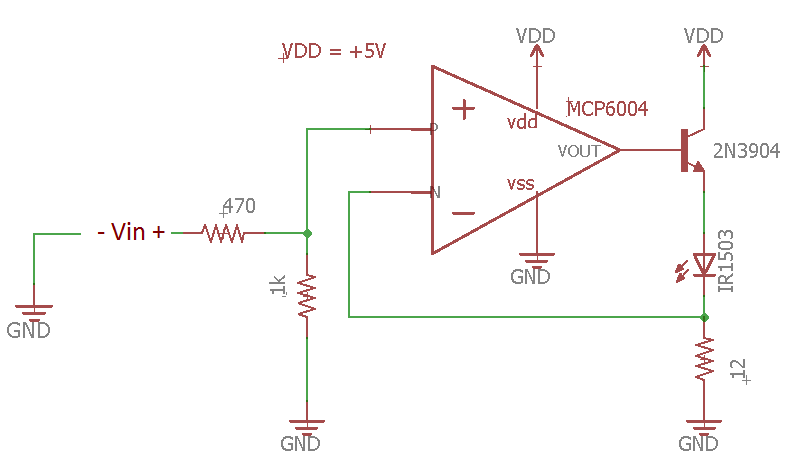
\includegraphics[width=0.6\linewidth]{ExperimentalImplementation/LEDDriverExperimentalSchem}
	\caption{Final schematic of current driver}
	\label{fig:leddriverexperimentalschem}
\end{figure}

The resulting output of current through the 12$\Omega$ resistor is shown in Figure \ref{fig:expcurrentlab4}.  The output from the current driver operated with at 20.1kHz with a 50.1\% duty-cycle.

\begin{figure}[H]
	\centering
	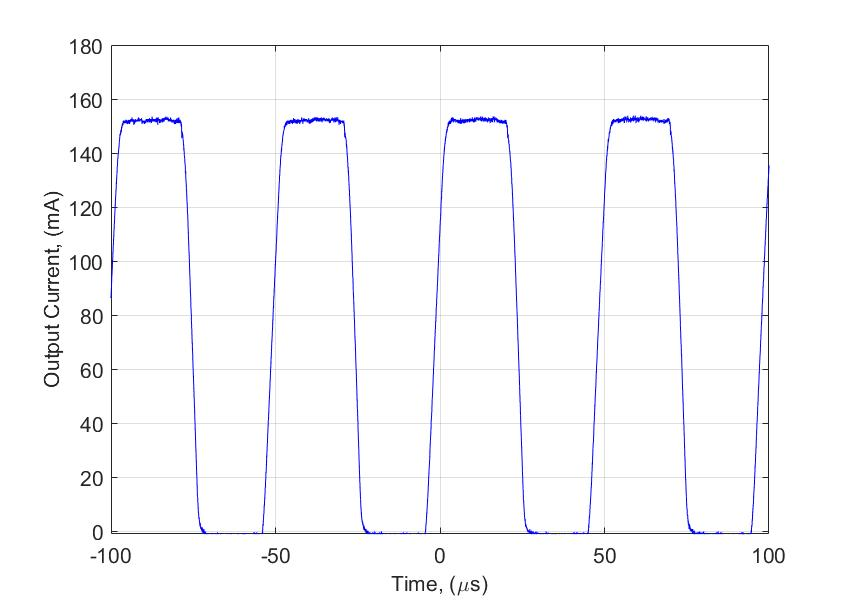
\includegraphics[width=0.6\linewidth]{ExperimentalImplementation/expcurrentlab4}
	\caption{Experimental output of current driver}
	\label{fig:expcurrentlab4}
\end{figure}

The experimental output differed from the simulated output shown in Figure \ref{fig:simcurrentlab4}. The greatest difference between them is the output current peak. The simulated peak current was $\approx$ 200mA, while the experimental output was $\approx$ 150mA. The duty cycle remains unaffected because the circuit allows it to be variable by adjusting the potentiometer depicted in the signal conditioner schematic, Figure \ref{fig:signalconditionerexperimentalschem}.   

\end{document}